\subsection{Sistema de Control}

En forma general, el sistema de control es el bloque de la plataforma que se encarga de tomar los datos de las señales medidas por los distintos sensores, convertirlos a una forma utilizable por el sistema, y luego, mediante un análisis de los mismos, generar señales de comando que se envían al convertidor para modificar su comportamiento, buscando llegar a un punto de funcionamiento adecuado para las condiciones existentes.\\

Todas estas tareas son llevadas a cabo por un dispositivo llamado {\Medium controlador digital de señales} o DSC (del inglés \textit{Digital Signal Controller}). Este dispositivo, como indica su nombre, es un microcontrolador convencional, pero que contiene ciertas modificaciones en su arquitectura de hardware y su repertorio de instrucciones (por ejemplo, hardware dedicado para la operación MAC o \textit{Multiply-and-Accumulate}) que lo adecuan para su uso en el procesamiento de señales digitales.\\

Además, los DSC suelen contar con una gran variedad de periféricos que les brindan flexibilidad para implementar las funcionalidades necesarias para los sistemas en los que se encuentran. Estos periféricos pueden ser módulos de comunicación de datos, contadores y timers, generadores de formas de onda, entre otras cosas. Esta combinación de procesador más periféricos de entrada/salida (y memoria), al implementarse en un sistema más grande y cumpliendo una función dedicada, como es el caso en esta plataforma, resulta en lo que se conoce como {\Medium sistema embebido}.\\

\subsubsection{Controlador Digital de Señales}

Para conformar el sistema embebido de control de la plataforma, se utiliza un controlador digital de señales perteneciente a la linea {\Medium C2000} de microcontroladores de tiempo real de Texas Instruments. En particular, se eligió el modelo {\Medium TMS320F28335} de arquitectura de bus tipo Harvard, \SI[]{150}{\mega\hertz} de frecuencia de reloj, CPU de 32 bits, memoria flash de 256K palabras de 16 bits, conversor analógico-digital de 12 bits y 16 canales, módulos de comunicación serie SPI, I\textsuperscript{2}C, y UART, entre múltiples otras funcionalidades.\textsuperscript{\cite{DSP-Datasheet}}\\

\begin{figure}[h]
    \centering
    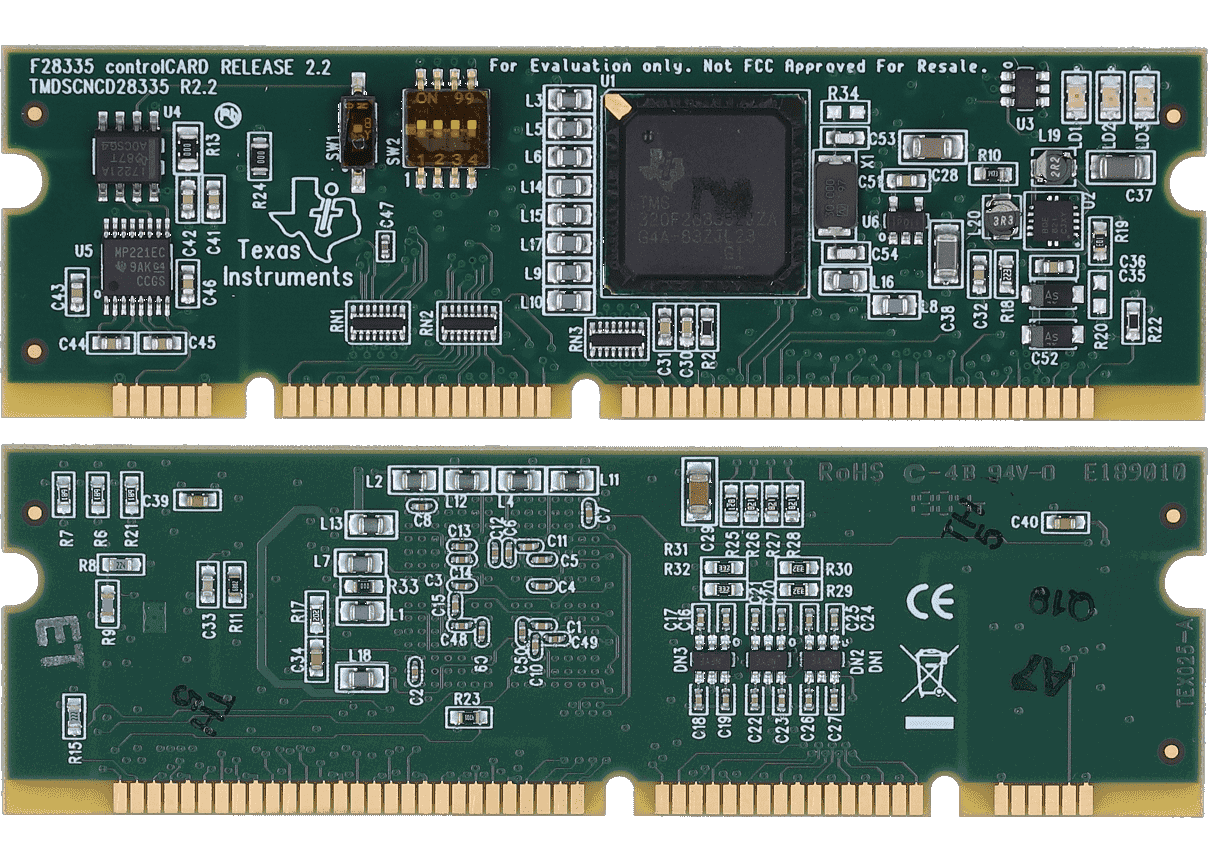
\includegraphics[scale=0.2]{Imagenes/ControlCARD.png}
    \caption{Controlador digital de señales modelo TMS320F28335 de la linea C2000, en su paquete de evaluación tipo ControlCARD, para inserción en slot DIMM-100.}
    \label{ControlCARD}
\end{figure}

Según la hoja de datos que provee el fabricante, este es un DSC optimizado para el procesamiento, sensado y actuación enfocado a mejorar el rendimiento en aplicaciones de control en tiempo real. Cuenta con una unidad de aritmética de punto fijo de 32 bits, además de una FPU (\textit{Floating-Point Unit}) de precisión simple de 32 bits, que le provee una flexibilidad para cumplir tareas tanto de microcontrolador convencional como de procesador de señales digitales. Como se mencionó arriba, tiene capacidad de procesamiento de MAC de 32 x 32 bits con resolución de salida de 64 bits.\textsuperscript{\cite{DSP-Datasheet}}\textsuperscript{\cite{DSP-TechManual}}\\

En tanto a los buses, al ser esta una arquitectura tipo Harvard, el dispositivo cuenta con tres buses separados: un bus de lectura de programa, un bus de lectura de datos y otro bus para la escritura de datos, ambos de 32 bits de ancho. Al estar todos separados, esto permite que se realice la lectura del programa, lectura de datos y escritura de datos en un único ciclo de reloj. Adicionalmente, cuenta con un bus de periféricos que se conecta mediante un \textit{bridge} o puente al bus de memoria principal.\textsuperscript{\cite{DSP-Datasheet}}\textsuperscript{\cite{DSP-TechManual}}\\

El DSC fue seleccionado principalmente por su disponibilidad en el laboratorio, además de que ya fue utilizado en otros proyectos que pueden ser usados como referencia a la hora de diseñar el módulo. En cualquier caso, basado en sus especificaciones, este controlador resulta apropiado para ser integrado al sistema, por su capacidad de procesamiento en tiempo real, su enorme cantidad y variedad de periféricos que permiten implementar diversas funcionalidades útiles, y su documentación muy completa por parte del fabricante.\\

\paragraph{Periféricos Importantes}

Entre la gran lista de periféricos de este dispositivo, se pueden destacar varios de ellos que nos van a resultar de particular interés para la implementación de la plataforma. Estos módulos se conectan a la memoria mediante el bus de periféricos, cada uno con su propio vector de interrupción. Estos son los módulos que nos van a servir principalmente para realizar la adquisición de datos de sensores y la generación de formas de onda de control.

\subparagraph{Módulo ePWM}

El módulo ePWM (\textit{Enhanced Pulse Width Modulator}) del TMS320F28335 cuenta con seis distintos canales de generación de formas de onda por modulación de ancho de pulso desde el ePWM1 hasta el ePWM6, cada uno con dos salidas PWM distintas, ePWMxA y ePWMxB. Todos estos módulos pueden ser unidos mediante un esquema de sincronización por reloj si se requiere que operen como un único sistema.\\

\begin{figure}[h]
    \centering
    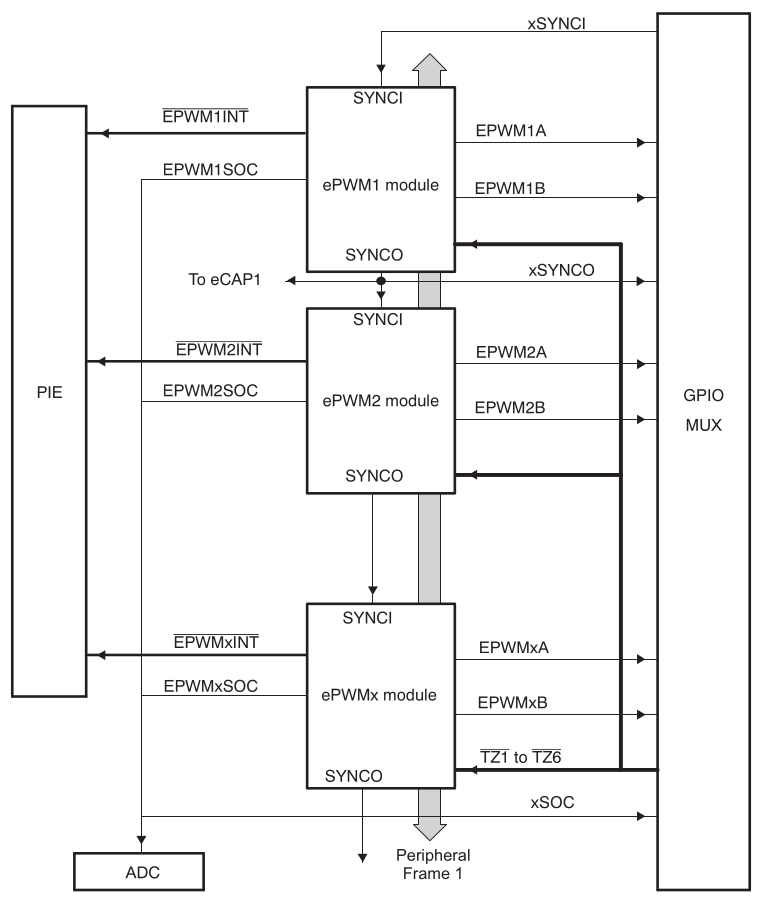
\includegraphics[scale=0.3]{Imagenes/Modulo ePWM.png}
    \caption{Diagrama de conexión interna de los módulos ePWM dentro del dispositivo.\textsuperscript{\cite{DSP-TechManual}}}
    \label{Modulo-ePWM}
\end{figure}

La frecuencia y fase de las ondas de cada uno de los módulos son controladas por un timer de 16 bits de longitud, con un \textit{prescaler} que permite modificar la base de tiempo mediante la división de frecuencia del reloj de entrada. Las salidas A y B de cada módulo se pueden configurar en tres modos: dos salidas independientes de operación flanco simple, dos salidas independientes de operación flanco dual simétricas, y una salida de operación flanco dual asimétrica.\\

Como se ve en la figura \ref{Modulo-ePWM}, cada módulo cuenta con una entrada de sincronización SYNCI y salida de sincronización SYNCO. Esto permite encadenar dos módulos, con la señal de sincronización de un módulo proveniente de otro módulo anterior. Además, cada módulo cuenta con un registro de fase de 16 bits, cuyo contenido define la fase de las ondas generadas respecto a las ondas del módulo del cual esta recibiendo la señal de sincronización (esto va a resultar útil para generar las señales de comando del convertidor full-brigde de la plataforma).\\

Adicionalmente, cada módulo ePWM cuenta con un submódulo de generación de banda muerta o \textit{dead-band} para flancos de subida y bajada. Esto permite generar un período de tiempo muerto (es decir, un tiempo en el que no se cambia de nivel) entre flancos de las salidas A y B del módulo. Esto resulta útil en convertidores puente, como función de seguridad para evitar el disparo simultáneo de las dos llaves de una pata.\textsuperscript{\cite{DSP-TechManual}}\\

\subparagraph{Módulo ADC}

El TMS320F28335 cuenta con un conversor analógico-digital de 12 bits (4096 niveles) de resolución y 16 canales, configurables como dos módulos independientes de 8 canales cada uno (ADCINAx y ADCINBx).\\

\begin{figure}[h]
    \centering
    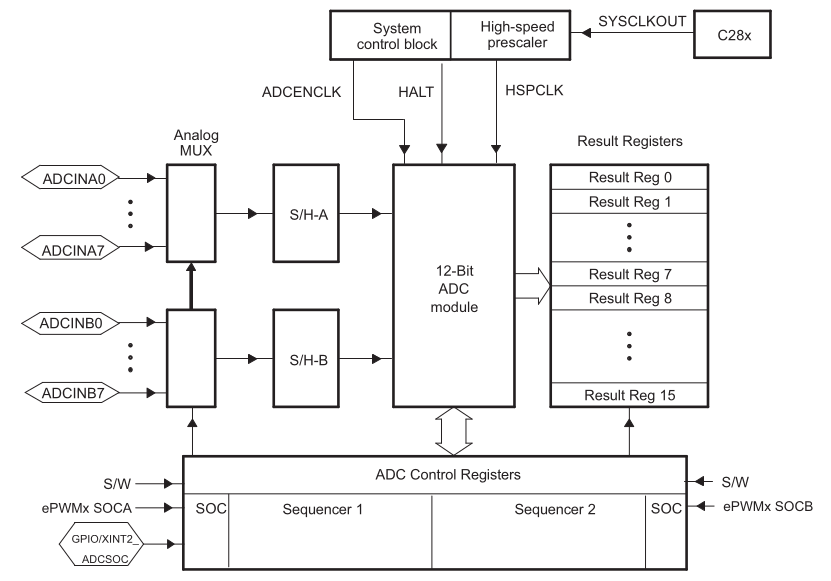
\includegraphics[scale=0.35]{Imagenes/Modulo ADC.png}
    \caption{Diagrama de la conexión interna del módulo de conversor analógico-digital del dispositivo.\textsuperscript{\cite{DSP-TechManual}}}
    \label{Modulo-ADC}
\end{figure}

Como se ve en la figura \ref{Modulo-ADC}, existe un único conversor en el cual las entradas analógicas ingresan a través de un circuito multiplexor analógico. Cada uno de estos multiplexores (uno para cada grupo A y B) tiene a continuación un circuito de \textit{Sample and Hold}, que se encarga de mantener el nivel de tensión de entrada fijo en el valor correspondiente al instante en el que se tomó la muestra para que se pueda realizar la conversión. Luego, el conversor toma valores de tensión entre \SI[]{0.0}{\volt} y \SI[]{3.0}{\volt}, convirtiendolos a una velocidad de \num[]{12.5} MSPS (período de conversión de \SI[]{80}{\nano\second}).\\

Además, existen múltiples posibles fuentes para la secuencia de inicio de conversión (SOC): inicio inmediato por software, inicio mediante señal ePWM, e inicio mediante la interrupción externa XINT2.\textsuperscript{\cite{DSP-Datasheet}}\\